\subsection{What is held out, and what still is not}
\label{sec:heldout}

\S\ref{sec:threats} concedes that three things were fitted to this corpus: grammar v2's
productions, the translator's feature vocabulary, and \S\ref{sec:staircase}'s
implementation order. Two of them are functions of the corpus and can therefore be
refitted --- take part of it, recompute the thing from that part alone, score it on the
rest. The third cannot. No script can produce the grammar we would have written had we
read half these dashboards, because those productions were added by hand in response to
what the corpus showed: that fit lives in the authors and not in a procedure. So the
vocabulary and the order are cross-validated here, and the grammar is tested the only way
it can be, on dashboards nobody involved in this work has read.

\paragraph{The vocabulary saturates long before the corpus ends.}
Splitting is by dashboard and never by query: queries inside one dashboard share a house
style, and letting them straddle the boundary would leak that style across it and flatter
every number below. Over $200$ replicates at each size, a vocabulary read off $28$ of the
$283$ Datadog dashboards holds $25.4$ of the corpus's $28$ features and already covers
$97.5\%$ ($\pm2.0$) of the queries in the $255$ it did not read; past $60\%$ of the
dashboards no replicate misses a feature at all. The PromQL side behaves the same way,
from a tenth of its $240$ dashboards to $21.3$ of $24$ features and $98.0\%$.
Figure~\ref{fig:heldout} is both curves. So the ceiling is not the artefact that paragraph
feared. \emph{Which features dashboards use} is answered by a small fraction of this
corpus, and the rest of it keeps confirming the answer rather than extending it --- which
is a fact about how few syntactic features dashboards draw on, and the same fact that
makes the staircase steep.

\paragraph{The build order survives being scored on dashboards it was not chosen from.}
Recomputing the greedy order on half the dashboards and scoring it on the other half
gives $89.9\%$ at sixteen features where the order's own half gives $90.9\%$ --- a gap of
one point. \S\ref{sec:discussion} calls the staircase the practical result of this paper,
and it is a claim about effort against coverage that survives the effort being spent in
an order chosen from somewhere else.

\paragraph{The grammar, on $497$ dashboards it has never seen.}
The corpus took the $200$ most-downloaded Prometheus dashboards from a catalogue that
now lists $5{,}904$ (\S\ref{sec:corpus}); the rest were never listed, downloaded or read.
\texttt{scripts/heldout\_fetch.py} takes every dashboard down to rank $700$ that the
corpus does not already hold, which is $500$ dashboards, $497$ of them carrying PromQL:
$16{,}569$ queries against the in-sample $7{,}286$, and $13{,}960$ distinct strings
against $6{,}040$. Table~\ref{tab:heldout} reports both beside each other. The in-sample
row is the Grafana part of the corpus alone, because comparing against
Table~\ref{tab:parse-coverage}'s PromQL row would confound the holdout with a change of
source: that row also carries kube-prometheus's jsonnet-compiled queries, which no
hand-built dashboard resembles. Measuring the Grafana part on its own reproduces that
table's whole PromQL residual of $58$, which is a check that this comparator is the
paper's own pipeline restricted and not a second one.

Dashboard-level disjointness is not string-level disjointness. A popular query recurs
across dashboards, so $1{,}438$ of the held-out strings are strings the corpus also
holds, and those are not held out in any sense that bears on a grammar; the rate that
belongs in this paper is the one on the $12{,}522$ whose instantiated form appears
nowhere in the corpus. There, frozen grammar v2 parses $99.6\%$, against $99.0\%$ on the
dashboards it was built from. It does not do worse out of sample. What does shrink is the
fit: v2 beats v1 by $1.2$ points in sample and by $0.8$ out of it, so about a third of
what the corpus-driven productions bought was specific to this corpus and about two
thirds of it was a gap in PromQL as people write it. That is the most precise statement
we can make about the largest of the three fits on the side where it can be tested, and
it is smaller than the paragraph it replaces assumed without saying.

The vocabulary result repeats out of sample exactly as the cross-validation predicts: the
$24$ features cover $100.0\%$ of those $16{,}569$ occurrences with none outside them, on
a population twice the corpus's size.

\paragraph{What the residual is, and why it is not cleaned up.}
Fifty distinct strings of $13{,}960$ defeat v2, and they are worth decomposing because
most of them are not PromQL. Two are Loki panels that \S\ref{sec:corpus}'s LogQL filter
failed to catch, six are VictoriaMetrics \texttt{WITH} templates, and $27$ use Grafana's
older \texttt{[[variable]]} interpolation, which \texttt{corpus.normalise} does not
instantiate because nothing in the corpus needed it --- an instantiation gap of ours
rather than a grammar gap. That leaves $15$ strings, about one in a thousand, that are
PromQL this grammar cannot parse. We report the rate as measured and do not remove the
other $35$ from it. Filtering a held-out population after seeing what it costs is how a
held-out set stops being one, and the dirt is itself a finding: a corpus of community
dashboards filed under one datasource contains several query languages, which the
curated $200$ understated.

\paragraph{The Datadog side, on a repository by other authors.}
An earlier version of this subsection reported the Datadog side as having only the second
remedy available --- a later commit of the same repository --- on the ground that no
second public body of Datadog dashboards exists to draw a disjoint set from. That was
wrong, and wrong about a repository in the same organisation with the same file layout.
\texttt{DataDog/integrations-extras} is the sibling of \texttt{integrations-core},
holding ``community developed integrations and plugins for the Datadog Agent'': $209$
dashboards shipped under the same \texttt{assets/dashboards/} path, read here by the same
extractor that read the corpus, and $139$ of them contribute the queries below. The
repository carries $3{,}073$ Datadog metric-query occurrences, of which $3{,}065$ in
$2{,}572$ distinct strings survive dropping every string whose instantiated form the
corpus already holds --- seven such forms, eight occurrences. Its formula layer, $265$
occurrences in $166$ forms, is set aside exactly as the corpus's $6{,}022$ are, because
no version of either grammar parses that language at all.
Table~\ref{tab:heldout}'s in-sample Datadog row is Table~\ref{tab:parse-coverage}'s own
\texttt{datadog} row recomputed by this script, down to the residual of $6$ --- a
stricter version of the check the Grafana comparator passes, which reproduces that
table's PromQL residual but not its row.

Frozen grammar v2 parses $99.9\%$ of those $2{,}572$ strings, which is its in-sample
rate, while v1 parses $94.4\%$ against $92.9\%$. The margin
\S\ref{sec:datadog-inference}'s corpus-driven productions bought therefore falls from
$7.0$ points to $5.6$. That is the strongest statement this design supports and it is
weaker than it looks: v2 does not fall at all, so there is no measurable overfit in v2 to
find, and the whole of the movement is v1 --- the \emph{unfitted} documentation grammar
--- doing better here than it does on the corpus. What the pair measures is a difference
between two populations read under the assumption that they are otherwise exchangeable.
The honest reading is that roughly four fifths of the climb reappears on dashboards the
grammar never saw.

The frozen translator, called exactly as \S\ref{sec:evaluation} calls it, returns
$\kappa=96.7\%$ of those $3{,}065$ occurrences against $96.6\%$ in sample, and $96.3\%$ of
the $2{,}564$ distinct instantiated forms against $96.5\%$. Those are not two results, one
up and one down. They are one result, which is that the two rates are indistinguishable.
Occurrences cluster inside dashboards --- $23$ of the $139$ carry any refusal at all, and
one integration's dashboard carries $30$ of them --- so dropping any single dashboard
moves the held-out figure anywhere in $96.7\%$ to $97.7\%$, where the same operation in
sample moves it only within $96.6\%$ to $97.0\%$. A tenth of a point sits well inside
that. What the comparison establishes is that nothing large is hiding on the Datadog
side, not that the fit is worth nothing.

\paragraph{The refusals out of sample are refusals the catalogue already names.}
What a held-out $\kappa$ can show that an in-sample one cannot is a failure mode nobody
had catalogued, and among the refusals there is none. The $98$ refused occurrences carry
four gap codes --- \textsc{phi\_quantile} $49$, \textsc{unsupported\_function} $40$,
\textsc{fill\_interpolation} $7$, \textsc{scope\_empty\_value} $2$ --- and all four are
families \S\ref{sec:gaps} names. The corpus raises a fifth, \textsc{scope\_disjunction},
which this repository does not, so what differs is a gap going unseen rather than a gap
appearing. The mixture differs less than it first appears, too:
\textsc{unsupported\_function} dominates in sample and here the quantile gap edges past
it, but $30$ of those $49$ occurrences are the one integration's panels, and without that
dashboard the in-sample order returns. \S\ref{sec:threats} argued that the shortfall was
structural rather than specific to this corpus with nothing but the shape of the gap
codes behind it. This is evidence for it.

Outside the refusals there is one new failure, and it is the only thing here the
catalogue did not predict. Two strings of $2{,}572$ do not parse, and they are one
construct: \texttt{stddev:} as a space aggregator, which no query in the corpus uses.
Being a parse failure rather than a typed refusal, it carries no gap code, so no reading
of the catalogue in sample could have anticipated it.

\paragraph{Two vocabularies, and the one that bounds $\kappa$.}
That construct is also the single feature the corpus's $28$ Datadog features do not have,
so the corpus vocabulary covers $99.9\%$ of these occurrences rather than all of them,
where the cross-validation above found no replicate missing a feature at all past $60\%$
of the corpus. But the set that bounds $\kappa$ is not that one. It is $S^\star$, the
$25$ features the translator demonstrably handles (\S\ref{sec:evaluation}), and
$S^\star$ covers $97.3\%$ of these occurrences --- the same $97.3\%$ it covers in sample
--- with $82$ occurrences outside it rather than two, under four features rather than
one. So the ceiling that matters reproduces out of sample to the decimal place, and it is
the smaller of the two numbers: reporting the $99.9\%$ as though it were the translator's
would overstate the reachable ceiling by $2.6$ points.

\paragraph{The later commit, now a check rather than the evidence.}
The second remedy still runs and is still reported, with its size attached. In the week
between the corpus commit and \texttt{c6cac33b42ac}, three dashboards changed in a way
that produced $99$ distinct query strings the corpus does not contain; frozen v2 parses
all $99$ and the frozen translator translates all $111$ of their occurrences with no
refusal. One hundred and eleven occurrences from three dashboards cannot estimate a rate
reported to a tenth of a point, and they are clustered besides. What the run establishes
is that a week of upstream change contained nothing this pipeline refuses, which is a
check against breakage, and re-running it against a commit a year from now costs nothing.

\paragraph{Where that leaves the threat.}
All three fitted things now have an out-of-sample reading. The vocabulary and the build
order are functions of the corpus and were refitted on part of it: the vocabulary
saturates after a tenth of the dashboards and the order loses one point --- and on the
disjoint repository the corpus vocabulary turns out to miss one aggregator after all. The
grammar is not refittable by any script, so it was frozen and run on populations nobody
here had read: $497$ community dashboards on the PromQL side, $99.6\%$ against $99.0\%$,
and a disjoint Datadog repository, $99.9\%$ against $99.9\%$. And $\kappa$ is $96.7\%$
out of sample against $96.6\%$ in it, on $3{,}065$ occurrences from $139$ dashboards by
other authors, refusing under four of the five families the catalogue already holds.

None of that makes $96.6\%$ a held-out estimate; it was obtained the way it was obtained.
What it does is bound the worry the estimate licenses. On every channel a script can
reach, the fit is worth at most a point, and on $\kappa$ the two readings differ by less
than the spread a single dashboard produces. Two caveats survive, and neither is leakage.
The first is authorship: \texttt{integrations-extras} is community- and partner-written,
which is the different-authors test, but those dashboards are built with the vendor's own
integration scaffolding against the vendor's own documentation, so their house style is
not independent of \texttt{integrations-core}'s --- \S\ref{sec:threats} puts a number on
how far it differs. The second is that string-level disjointness is not structural
novelty. Nothing in this population survives even whitespace- and tag-order-blind
matching against the corpus, and yet $90.0\%$ of its occurrences have a feature set that
occurs there verbatim: these are largely the same query shapes over different metrics,
which is what a grammar is tested by and not what a body of unfamiliar practice would
be. So \S\ref{sec:threats}'s preference for private, customer-written dashboards stands
unmet. It is the one test this paper cannot run rather than the one it declined to.

\begin{figure}[htbp]\centering
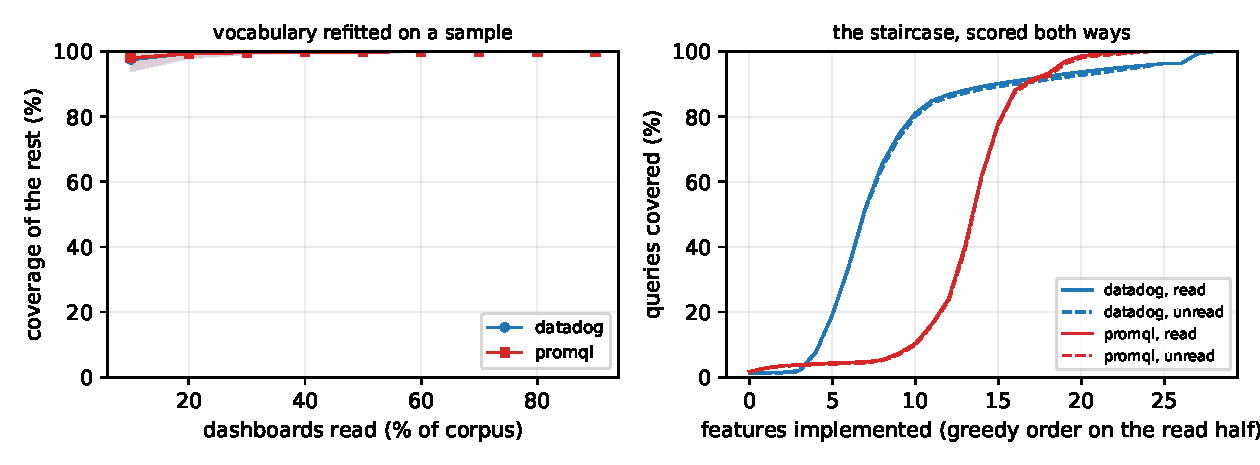
\includegraphics[width=0.92\linewidth]{figures/heldout_vocabulary}
\caption{Refitting the two things that are functions of the corpus. Left: a feature
vocabulary read off a sample of the dashboards, scored on the dashboards it did not read;
the band is the $5$th to $95$th percentile over $200$ replicates. Right: the greedy
implementation order recomputed on half the dashboards, scored on both halves. Neither
panel is a held-out $\kappa$ --- they bound the ceiling and the build order, which are
the parts of the fit a script can undo.}
\label{fig:heldout}
\end{figure}

\begin{table}[htbp]\centering\footnotesize
\begin{tabular}{@{}lrrrrrr@{}}
\toprule
Population & Queries & Distinct & Raw & v1 & v2 & Residual \\
\midrule
Grafana, the corpus's $199$ & 7,286 & 6,040 & 71.0\% & 97.8\% & 99.0\% & 58 \\
Grafana, $497$ it never saw & 16,569 & 13,960 & 77.5\% & 98.7\% & 99.6\% & 50 \\
\quad its strings the corpus lacks & --- & 12,522 & --- & 98.8\% & 99.6\% & --- \\
\texttt{integrations-core}, the corpus's $283$ & 8,770 & 7,799 & 11.8\% & 92.9\% & 99.9\% & 6 \\
\texttt{integrations-extras}, $139$ others & 3,065 & 2,572 & 22.8\% & 94.4\% & 99.9\% & 2 \\
\texttt{integrations-core}, $3$ at a later commit & 111 & 99 & 1.0\% & 100.0\% & 100.0\% & 0 \\
\bottomrule
\end{tabular}

\caption{The frozen grammars inside and outside the corpus. ``Raw'' is the share of
distinct queries that parse as shipped; the v1 and v2 columns are after template
instantiation, as in Table~\ref{tab:parse-coverage}, and the residual is what v2 still
cannot parse. The one indented row restricts the row above it, to the strings
whose instantiated form the corpus does not hold, which is the comparison the text
quotes; the Datadog rows are four separate populations and none of them is nested in
another. \texttt{integrations-extras} is the disjoint repository, every string of which
is one the corpus does not hold. The last row is \texttt{integrations-core} at a later
commit, which holds only strings the corpus lacks and at $99$ of them estimates
nothing.}
\label{tab:heldout}
\end{table}
